\title{G54MRT Coursework 2 - The Ergonomotron}
\author{
  Jack Ellis \\
  psyje5@nottingham.ac.uk\\
  4262333\\\\
}
\date{}
\documentclass[12pt, a4paper]{report}
\usepackage{graphicx}
\graphicspath{{Images/}}

\usepackage{listings}
\lstset{
   basicstyle=\ttfamily\tiny
  ,language=Python
  ,showstringspaces=false
}



\begin{document}
\maketitle

\tableofcontents
\pagebreak

\section{Summary}
The broad idea of this project is to ensure a user is sitting properly and comfortably at their computer.
The project will use a combination of light sensors, and accelerometers to detect first whether or not the user is looking at their screen, and second whether or not they are craning their neck to do so in such a way as would lead to long-term damage.

\section{Background and Motivation}
Prolonged viewing of a computer screen can lead to many problems with regard to eye health, including dry eye syndrome\cite{dryeyes}, a condition in which the eyes do not produce enough tears, leading to irritation.
"Back and neck pain, headaches, and shoulder and arm pain are common computer-related injuries."\cite{vicgov}, and are related to poor posture when a user is at their workstation.
This project aims to alleviate these issues using a combination of light sensors and a 3-axis accelerometer.
The intended setting is, ultimately, in the workplace.
Many office jobs require employees to be sat at computers for large amounts of time, with no proper enforcement of regular breaks to ensure employee health.

\section{Related Work}
There is a lot of work currently centered around making computers more ergonomic and healthier to use, including standing desks, the adoption of blue light filters in software, and various monitor and laptop stands designed to raise the device screen such that the user is not craning their neck down risking damage.

\section{Design}

The system is designed around 3 sensors: 2 light sensors, and a 3-axis gyroscope/accelerometer.
The light sensors will be arranged vertically at the front of the headgear, with a divider in between them to give an "above/beneath" light reading.
The gyroscope will be mounted wherever is convenient on the headgear.
Figure \ref{fig:diagram} shows the connections that will be made.

\begin{figure}
  \centering
  \caption{A diagram showing the connections}
  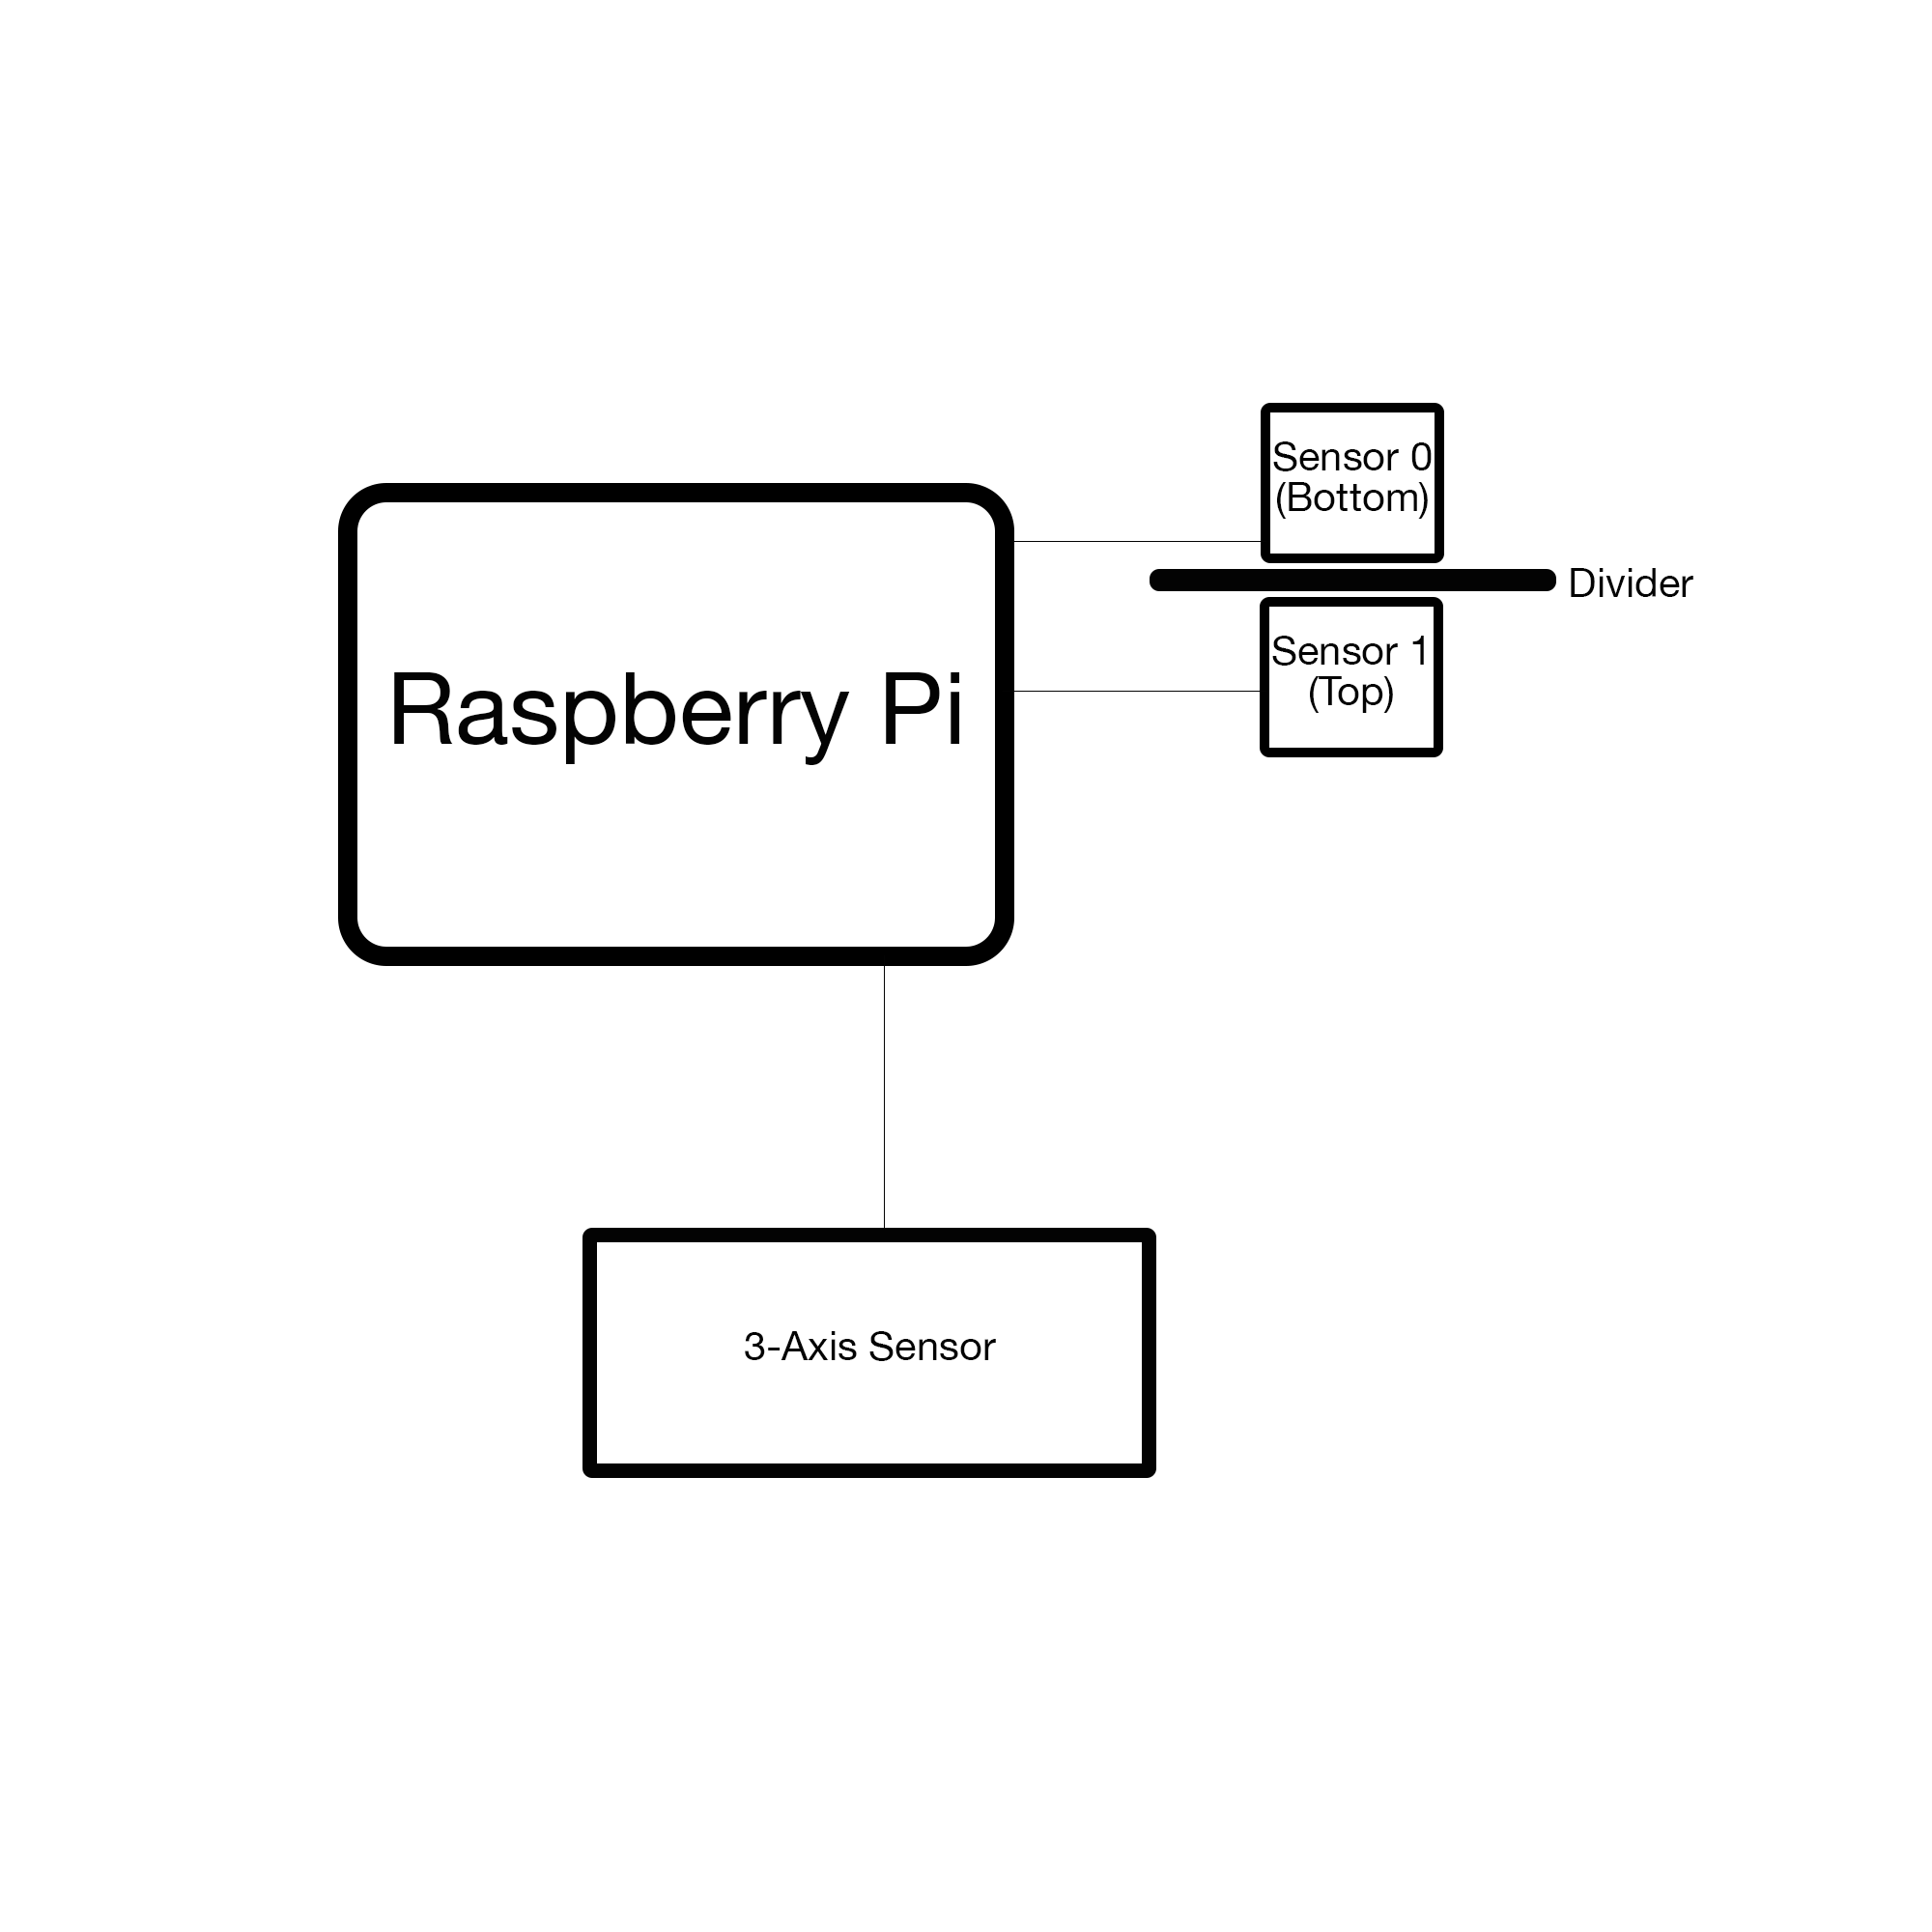
\includegraphics[width=1\textwidth]{Diagram.png}
  \label{fig:diagram}
\end{figure}


\section{Implementation}

The prototype is based around a baseball cap, with the peak acting as the divider.
The sensors are attached using bent paperclips, and the Raspberry Pi is mounted to the top of the hat.
One light sensor is mounted above the peak, and the other hangs below it, while the gyroscope is mounted to the side of the hat, as shown in the photo in Figure \ref{fig:hatpic}.

\begin{figure}
  \centering
  \caption{The prototype}
  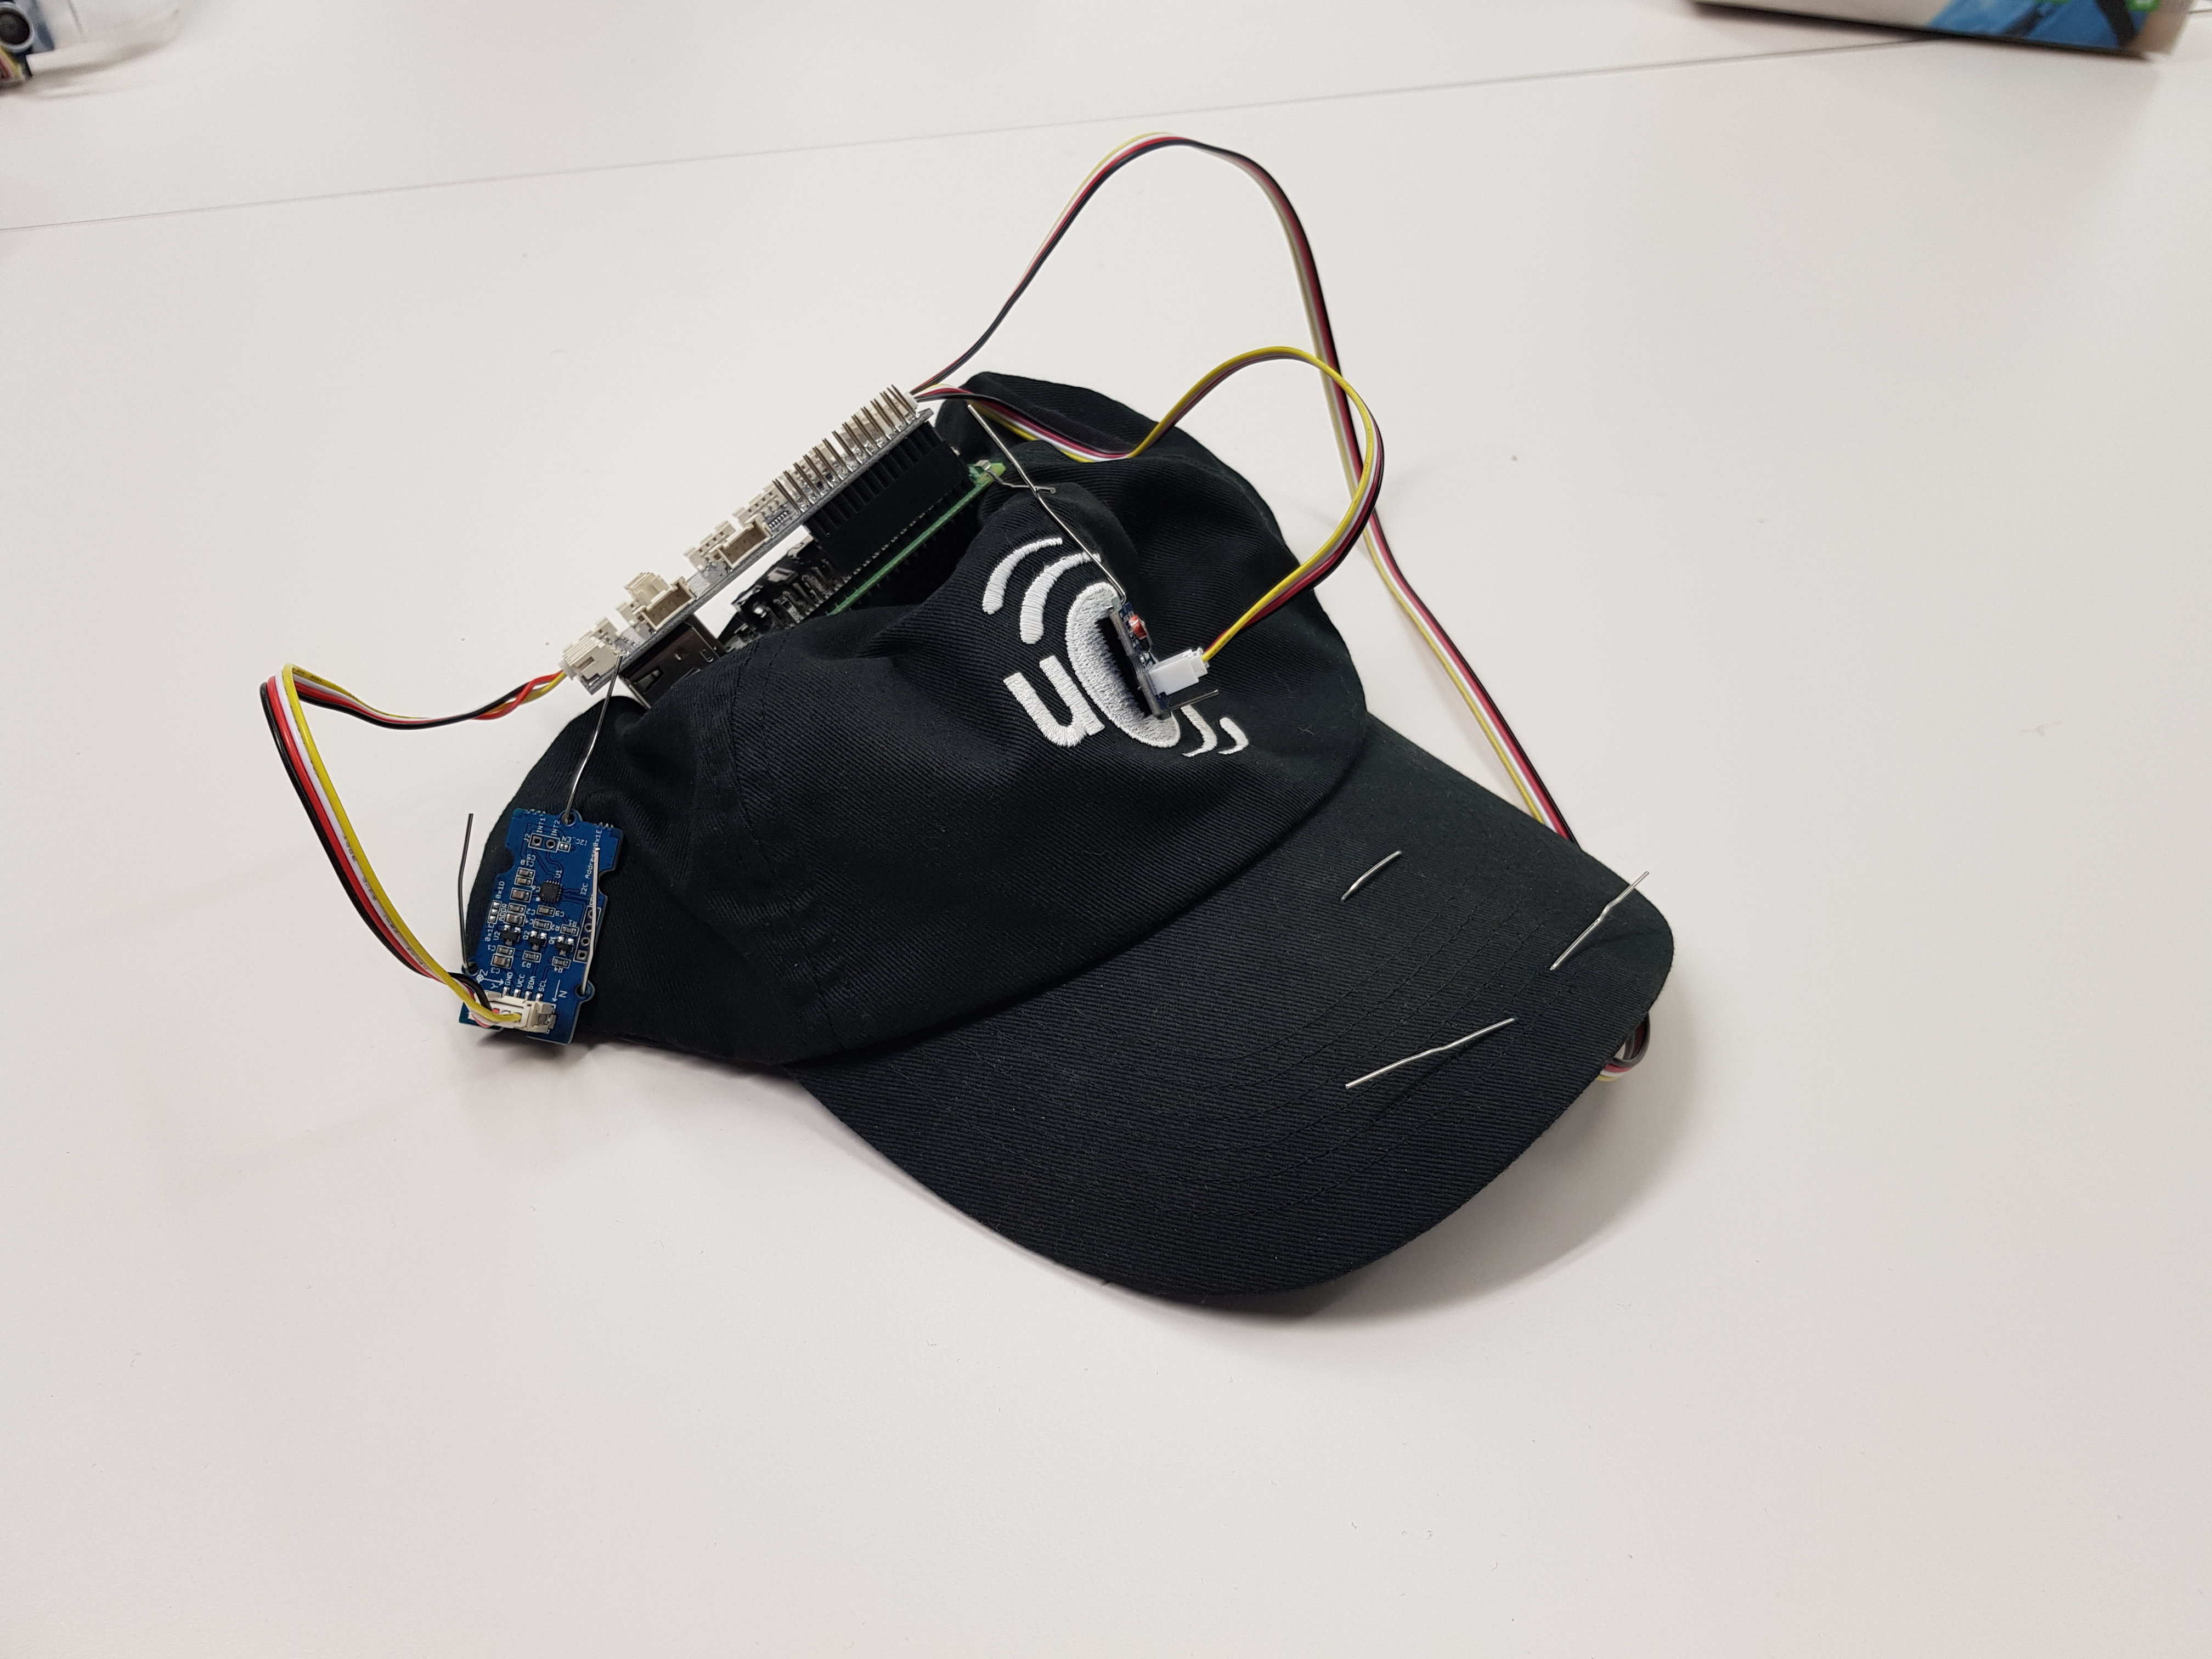
\includegraphics[width=1\textwidth]{hatpic.jpg}
  \label{fig:hatpic}
\end{figure}

\par

The code is split into three main sections: the calibration phase and the actual real-time sensing phase.

\subsection{Setup}

This takes place outside of the main \verb|while| loop, and will declare all used variables and functions within the code.

First \verb|time| and \verb|math| (as well as the grovepi modules) are imported.
This is to allow for tracking of the duration of certain events and to allow the value of \verb|pi| to be used in angle calculations.

\par

Next a number of global variables are declared.
The main timer, \verb|t|, is set to 0, and the initial values for the low-pass filters on both the difference in light levels and the angle of neck lean are set, to 0 and $\pi/2$ respectively.
Finally the variables for the calibration phase are initialised - \verb|calibrationPassesInit| is set to 100 (there will be 100 passes of calibration, this can be adjusted as deemed necessary), and \verb|calibrationPasses| is set to the value of \verb|calibrationPassesInit|.
The accumulator values that will be used to calibrate both light sensors are set to 0.

\lstinputlisting[firstline=10,lastline=21,caption=Setting up variables]{../sensors.py}

\subsection{Calibration}

Initially there are two variables, \verb|calibrationPassesInit| and \verb|calibrationPasses|.
These are both set to 100, which will be the number of times the sensors take data with which to calibrate themselves to the light levels in the rest of the room.
This corresponds to roughly 10 seconds of reading.

\par

The light levels are stored in variables, with the values being accumulated over the number of passes, and once the counter (as defined by \verb|calibrationPasses|) reaches 0, that value is divided by the initial number of passes (defined by \verb|calibrationPassesInit|), to give an average value for the light level in the room both above and below the divider.

\lstinputlisting[firstline=29,lastline=45,caption=Calibration Phases]{../sensors.py}

\subsection{Real-Time Sensing}

Once the calibration phase is completed, the real time sensing of light levels and neck angle begins.
The light values from the sensors have the values calculated by the calibration phase subtracted from them, and the relative difference between the fixed values of the top and bottom sensor calculated.
Finally for this section, a low-pass filter is applied to this difference such that the user cannot quickly move their head and reset the timer (the timer will be discussed later).

\lstinputlisting[firstline=47,lastline=54,caption=Calculating the difference between sensor values]{../sensors.py}

\par

The neck angle is then taken and a low-pass filter applied similar to the process for the light sensors.

\lstinputlisting[firstline=60,lastline=63,caption=Calculating the neck angle]{../sensors.py}

\subsection{Processing}

In this phase it is first determined whether or not the difference between top and bottom sensors is more than a factor of 1.2 (i.e. whether or not the bottom sensor value is more than 1.2 times the top sensor value).
If it is, the user is deemed to be looking at a screen, and the timer has 0.1 added to it (this roughly corresponds to the number of seconds between each sensor reading).
If the timer reaches the value of \verb|problemTime|, defined before the main loop begins, it prints a message instructing the user to look away from the screen.
While this goes on, the value of the user's neck angle is monitored, and if it exceeds the value of \verb|problemAngle|, again defined outside of the main loop, it will print a different error message instructing the user to lean their head back.
If the user is not deemed to be looking at a screen the timer resets.

\lstinputlisting[firstline=66,lastline=77,caption=Processing and printing the data]{../sensors.py}

\section{Testing}

Testing the system consisted of attempting to use the system and determining whether or not looking at a screen was detected at all.
The testing was also an opportunity to fine-tune the threshold values for said determination, as well as the method by which the difference was calculated.

\par

Initially the difference was calculated as an absolute value, i.e. the value of one sensor minus that of the other, however in testing in rooms of varying ambient light intensities it was found that this did not work - a brighter room would result in false negatives.
Adjusting the code to use a relative difference, i.e. the value of one sensor \textit{over} that of the other, made the code work considerably more effectively.

\par

Once this "calibration" testing was done I set about testing the system in a variety of scenarios: light room, dark room, and with different types of screens (phone, laptop, desktop).
In all cases it successfully determined when I was looking at a screen, and whether or not my neck was at an excessive angle.
In some cases however the neck tilt was such that both light sensors were aimed at the screen in use, consequently the system failed to register the excessive angle.
In a future revision I would invert the order of the if statements - detect the neck tilt regardless of the light level and alert the user of excessive neck angle whether or not they are looking at a screen.

\section{Critical Reflection}

Overall I am happy with the system, as stated in the previous section I would change the order of "event priority", neck tilt taking precedence over looking at a screen.
The system works well in my view however the initial prototype is very clunky, not to mention quite heavy, which will exacerbate any neck-tilt issues as the user must contend with the weight of the device.
Having the user tied to a desk via the Pi's USB lead or having to carry around a battery pack is also not ideal, but this is only a prototype and consequently the finished system would be somewhat more refined.

\par

There is scope for further enhancement; additional sensors to detect the distance from the user to the screen would be the next logical step, with the "problem time" value becoming a factor of this distance.

\par

Broadly speaking however I feel that this project has done what it set out to do very well.

\begin{thebibliography}{0}
  \bibitem{dryeyes}
    \textit{Office screen work linked to dry eye syndrome}, 2014-06-18\\
    www.nhs.uk/news/lifestyle-and-exercise/office-screen-work-linked-to-dry-eye-syndrome\\
    Accessed 2018-03-08
  \bibitem{vicgov}
    \textit{Computer-related injuries}\\
    www.betterhealth.vic.gov.au/health/healthyliving/computer-related-injuries\\
    Accessed 2018-03-08
\end{thebibliography}

\appendix

\section*{Appendix A - Instructions for setup/running}

This will assume you are using the prototype hat seen in Figure \ref{fig:hatpic}.

\begin{enumerate}
  \item Connect an LED screen to the Raspberry Pi - this can be disconnected later however it is needed so as to ascertain the IP address of the Pi.
  \item Connect the Raspberry Pi to power.
  \item From an SSH client connect to the Pi using the IP address on the LED screen, logging in as user \verb|g54mrt|.
  \item Disconnect the LED screen.
  \item Copy \verb|sensors.py| to the root folder of the user \verb|g54mrt|.
  \item Run the command \verb|python sensors.py|.
  \item The program will run. To terminate the program press control-C.
\end{enumerate}

\end{document}
